\documentclass[12pt]{beamer}

\usepackage[T1]{fontenc}
\usepackage[utf8]{inputenc}
\usepackage[english]{babel}
\usepackage{mathtools}
\usepackage{amsthm}
\usepackage{libertine}
\usepackage[libertine]{newtxmath}
\usepackage[mathscr]{euscript}
\usepackage{tikz-cd}
\usetikzlibrary{decorations.markings}
\usepackage{float}
\usepackage{listings}
\usepackage{xcolor}
\usepackage{booktabs}

\usepackage[scaled=0.9]{inconsolata}


%% ------------- Beamer style settings -------------
%\usefonttheme{serif}
\usetheme{Singapore}
\usecolortheme{rose}

%Deactivating navigation symbols
\setbeamertemplate{navigation symbols}{}


% Deactivate the shading at the top of slide
% \newcommand{\removeheadshading}[0]{%
% 	\setbeamertemplate{headline}{%
% 		\begin{beamercolorbox}{section in head/foot}%
% 			\vskip2pt\insertnavigation{\paperwidth}\vskip2pt%
% 		\end{beamercolorbox}%
% 	}%
% }
% \removeheadshading
\setbeamertemplate{headline}{}


%% ------------- Math commands -------------
% New math commands
\DeclareMathOperator{\img}{Im}
\DeclareMathOperator{\sign}{sign}
\DeclareMathOperator{\id}{Id}
\DeclareMathOperator{\vol}{vol}
\DeclareMathOperator{\hodgestar}{\ast}
\DeclareMathOperator{\Hom}{Hom}

\newcommand{\interior}[1]{{\kern0pt#1}^{\mathrm{o}}}
\newcommand{\into}{\hookrightarrow}
\newcommand{\onto}{\twoheadrightarrow}
\newcommand{\opartial}{{\overline{\partial}}}

%% ---------------- Code design --------------------
\definecolor{codebg}{RGB}{245,245,245}
\definecolor{codeblue}{RGB}{36,36,140}
\definecolor{codegreen}{RGB}{0,120,0}

\lstset{
    backgroundcolor=\color{codebg},
    basicstyle=\ttfamily\small,
    keywordstyle=\color{codeblue}\bfseries,
    commentstyle=\color{codegreen},
    stringstyle=\color{red},
    frame=single,
    rulecolor=\color{black!20},
    breaklines=true,
    showstringspaces=false,
    tabsize=4
}

%% ------------- Settings fpr document -------------
\title[Minimum Lap-Time Optimization]{Minimum Lap-Time Optimization of a Racing Line Using Optimal Control}
\author{Álvaro Galisteo Bermúdez, Daniel Rath, Anastasiia Kliushnik}
%\institute{Albert-Ludwigs-Universit\"{a}t Freiburg}
\date{21.07.2026}

\makeatletter
\hypersetup{
	pdftitle={\@title},
	colorlinks,
	linkcolor=[rgb]{0.2,0.2,0.6},
	citecolor=[rgb]{0.2,0.6,0.2},
	urlcolor=[rgb]{0.6,0.2,0.2}}
\makeatother

\begin{document}

	% Title Page
	\frame{\titlepage}

    \begin{frame}{Problem Formulation}
    \begin{block}{Objective}
        \[
            \min_{T,\,z(\cdot),\,u(\cdot)} T
        \]
    \end{block}
    \small
    \begin{columns}[T,onlytextwidth]
        \column{0.46\textwidth}
        \textbf{States and controls}
        \[
            z=
            \begin{bmatrix}
                s & e_y & e_\psi & v
            \end{bmatrix}^{T}
        \]
        \[
            u=
            \begin{bmatrix}
                a & \delta
            \end{bmatrix}^{T}
        \]
        \scriptsize
        \[
        \begin{aligned}
            s &: \text{track progress},\\
            e_y &: \text{lateral offset},\\
            e_\psi &: \text{heading error},\\
            v &: \text{velocity},\\
            a &: \text{longitudinal acceleration},\\
            \delta &: \text{steering angle}.
        \end{aligned}
        \]
        \column{0.52\textwidth}
        \textbf{Vehicle dynamics}
        \[
        \begin{aligned}
            \dot{s}
            &=
            \frac{v\cos(e_\psi)}
            {1-\kappa e_y},
            \\[0.15cm]
            \dot{e}_y
            &=
            v\sin(e_\psi),
            \\[0.15cm]
            \dot{e}_\psi
            &=
            \frac{v}{L}\tan(\delta)
            -
            \kappa\dot{s},
            \\[0.15cm]
            \dot{v}
            &=a.
        \end{aligned}
        \]
    \end{columns}
    \end{frame}

    \begin{frame}{Physical and Track Constraints}
    \small
    \begin{columns}[T,onlytextwidth]
        \column{0.48\textwidth}
        \textbf{Track boundaries}
        \[
            -e_{y,\max} \leq e_y \leq e_{y,\max}
        \]
        \vspace{0.3cm}
        \textbf{Velocity}
        \[
            0 \leq v \leq v_{\max}
        \]
        \vspace{0.3cm}
        \textbf{Longitudinal acceleration}
        \[
            a_{\min} \leq a \leq a_{\max}
        \]
        \column{0.48\textwidth}
        \textbf{Steering}
        \[
            -\delta_{\max} \leq \delta \leq \delta_{\max}
        \]
        \vspace{0.3cm}
        \textbf{Lateral acceleration}
        \[
            \left|
            \frac{v^2}{L}\tan(\delta)
            \right|
            \leq a_{y,\max}
        \]
        \vspace{0.3cm}
        \textbf{Frenet validity}
        \[
            1-\kappa e_y > 0
        \]
    \end{columns}
    \end{frame}

    \begin{frame}{Numerical Solution}
    \small
    \begin{block}{Direct multiple shooting}
    \[
        Z_{k+1}=F_{\mathrm{RK4}}(Z_k,U_k,\Delta t),
        \qquad
        \Delta t=\frac{T}{N}
    \]
    \end{block}
    \begin{itemize}
        \item The lap is divided into \(N=200\) shooting intervals.
        \item The states \(Z_k\) are optimized at every node.
        \item Vehicle dynamics are integrated with RK4.
        \item The resulting NLP is built in CasADi and solved with IPOPT.
    \end{itemize}
    \end{frame}

    \begin{frame}{Optimized Trajectory}
        \centering
        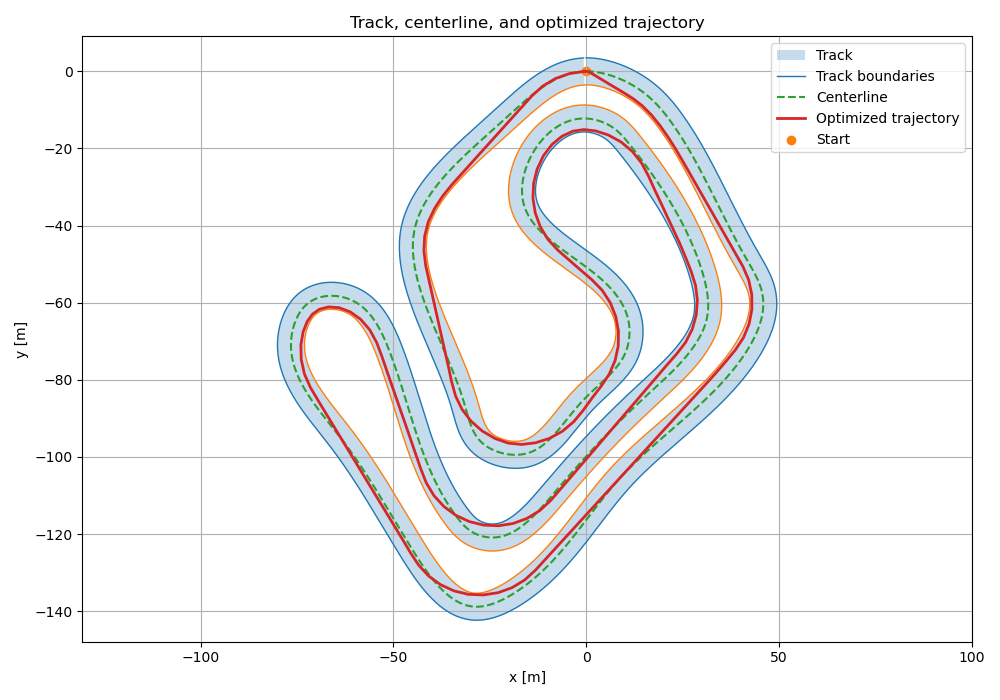
\includegraphics[
        width=0.90\textwidth,
        height=0.72\textheight,
        keepaspectratio
        ]{images/track_optimzed_traj.png}
        \vspace{0.1cm}
        \small
        \\
        The optimized path uses the available track width to increase the effective cornering radius.
    \end{frame}

    \begin{frame}{Results}
    \begin{columns}[T,onlytextwidth]
        \column{0.58\textwidth}
        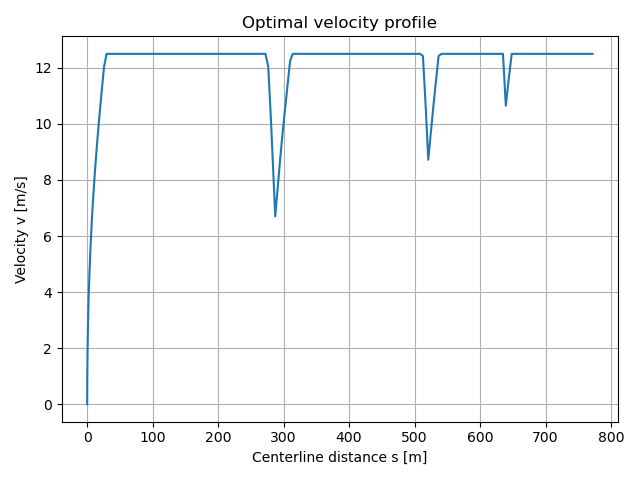
\includegraphics[
            width=\linewidth,
            height=0.55\textheight,
            keepaspectratio
        ]{images/vel_profile.png}
        \small
        The kart reaches the speed limit on most straights and slows down in the high-curvature sections.
        \column{0.38\textwidth}
        \vspace{0.6cm}
        \small
        \begin{tabular}{@{}lr@{}}
            \toprule
            Quantity & Value \\
            \midrule
            Lap time & \(61.665~\mathrm{s}\) \\
            Maximum speed & \(12.5~\mathrm{m/s}\) \\
            Maximum offset & \(2.87~\mathrm{m}\) \\
            IPOPT iterations & \(357\) \\
            Solver time & \(8.0~\mathrm{s}\) \\
            \bottomrule
        \end{tabular}
    \end{columns}
    \end{frame}

    \begin{frame}{Extension: Static Obstacle Avoidance}
        \centering
        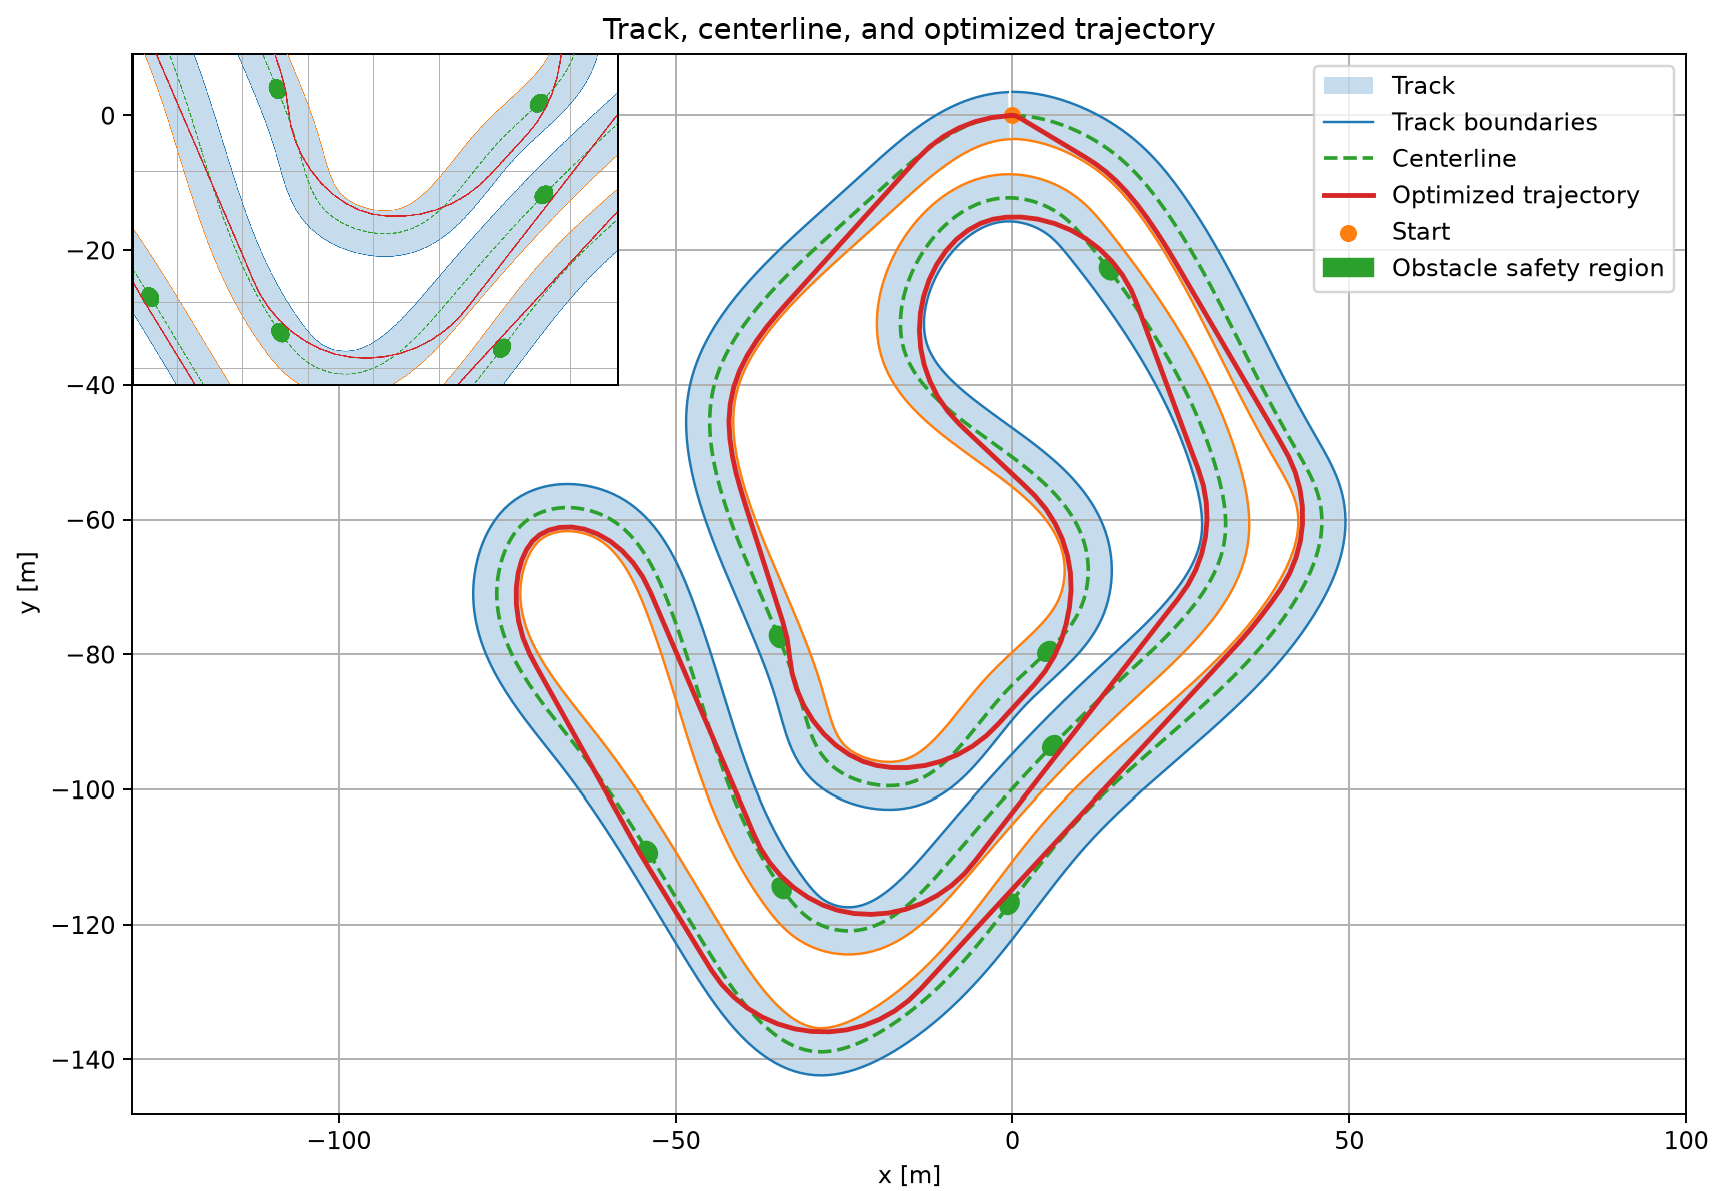
\includegraphics[
        width=0.90\textwidth,
        height=0.72\textheight,
        keepaspectratio
        ]{images/track_optimzed_traj_obst.png}
        \vspace{0.1cm}
        \small
        \\
        The optimized trajectory deviates only locally to avoid the obstacles, increasing the lap time from \(61.665~\mathrm{s}\) to \(61.800~\mathrm{s}\).
    \end{frame}

    \begin{frame}{Conclusions}
    \begin{itemize}
        \item The optimal control problem was successfully solved using direct multiple shooting.
        \item The optimized trajectory uses almost the full available track width.
        \item The kart reaches the maximum speed on the straights and slows down in the most demanding corners.
        \item The resulting minimum lap time is \(61.665~\mathrm{s}\).
        \item The proposed formulation was successfully extended to include static obstacle avoidance.
    \end{itemize}
    \vspace{0.3cm}
    \begin{block}{Main result}
        Optimal control provides a feasible racing line that minimizes the lap time while satisfying the vehicle and track constraints.
    \end{block}
    \end{frame}
        
\end{document}